\documentclass[letterpaper, 12 pt, conference]{ieeeconf}

\usepackage{siunitx}
\usepackage{graphicx}
\usepackage[utf8]{inputenc}
\usepackage[T1]{fontenc}
\usepackage{subfigure, siunitx, url}
\usepackage{amsmath, amssymb, bbm, nicefrac}
\usepackage{pifont}
%\usepackage{tikz}
%\usetikzlibrary{shapes,arrows,fit,trees,positioning,chains,calc,intersections}

%%% abbreviations to use (guarantee correct spaces between characters)
\newcommand{\ie}{i.e.\ }
\newcommand{\Ie}{I.e.\ }
\newcommand{\eg}{e.g.\ }
\newcommand{\Eg}{E.g.\ }
\newcommand{\cf}{cf.}

%%% commands for referencing (guarantee homogeneous writing style)
\newcommand{\referenceChapter}[1]{Chapter \ref{#1}}
\newcommand{\referenceSection}[1]{Section \ref{#1}}
\newcommand{\referenceFigure}[1]{Figure \ref{#1}}
\newcommand{\referenceEquation}[1]{Eq.~(\ref{#1})}
\newcommand{\referenceTable}[1]{Table \ref{#1}}
\newcommand{\referenceListing}[1]{code listing\ref{#1}}
\newcommand{\referenceAlgorithm}[1]{Algorithm \ref{#1}}

\title{\LARGE \bf
Towards the Goal \\ \small Machine Learning 4155 Final Project Paper
}


\author{Alexander Moriarty\\~\\~
		Faculty of Computer Science, Dalhousie University\\ 
        6050 University Ave, Halifax, Nova Scotia, Canada\\
        {\tt\small moriarty@cs.dal.ca}
}

\begin{document}

\maketitle

\begin{abstract}
The purpose of this lab was to investigate the use of the Proportional Integral Derivative controller algorithm in a wall-following robot exercise. A Proportional Integral Derivative controller, also known as a PID controller, utilizes the variance between the desired state of the function and the actual state of the function (the robot's behaviour being the function in this case) and is represented by \referenceEquation{pid-function}.
\end{abstract}

\section{Introduction}
\label{section::introduction}

The task at hand involved programming a robot to navigate to a goal on top of a table while avoiding obstacles and the edge. The system had to be responsive to changes in the environment, as the obstacles were not necessarily stationary. Machine learning techniques\cite{ttml} were incorporated to achieve a flexible and robust solution that would improve as the robot moved towards the goal. The sensors incorporated were: a standard definition webcam, ultrasonic distance sensor, light sensor and touch sensor. The camera was placed over the table to determine the position and orientation of the robot, the goal, and drivable regions. The light and touch sensors on the NXT were the backup sensors for avoiding the table edge and objects, respectively. The ultrasonic sensor was mounted on a servomotor to enable a check of multiple directions and incorporate the different distance measures into our overall controller.

\section{Hardware \& Software Platform}
\label{section::platform}

The robot was a Lego NXT tribot, two notable modifications were made.  First, mounting a third servomotor to allow the forward facing ultrasonic sensor to rotate. Second, coloured blobs were mounted above the front and rear of the robot to simplify the detection and calculate the direction of the robot. The project relied on Python, nxt-python\footnote{\url{http://code.google.com/p/nxt-python}}  and OpenCV\footnote{\url{http://opencv.org/}}  (versions 2.7.2, 2.2, 2.4.3 respectively). Development and testing was completed using software across Linux, Windows and Mac with different webcams without experiencing any added difficulty. Scikit-Learn was considered, to learn a function to translate from camera data to the robot's orientation.  This option was determined to be unnecessary because calculation of robot’s direction was done analytically with trigonometry.
\section{Controller Architecture}
\label{section::controller}

The overall solution was divided into smaller tasks, which would work well in parallel. The aim was to have all of the processes running in parallel and then combine them together in order to decide which action to take given the robots current perceived location. We also included past data and the robot’s history through a Proportional-Integral-Derivative (PID) controller. In the final implementation, the sub processes ran in a pseudo parallel manor. The processes ran in sequence, but independently of each other.  The results were all taken into account as if they had been run in parallel. This decision was made due to time constraints and not knowing the technical nuances of python multiprocessing. A purely parallel implementation would likely be faster. At the beginning of each step, the robot locates itself which requires grabbing several frames from the webcam and discarding the first few because the camera has autofocus and colour filters that cannot be turned off. If the OpenCV components could be run in parallel, the location and orientation of the robot could be queried at any time without waiting for the camera to re adjust and grabbing unnecessary frames.

\section{Perception \& Computer Vision}
\label{section::perception}

The OpenCV library was used to interface with the webcam. The latest major build of OpenCV stores image data as numpy arrays. This allows for simplified processing and iterating through the image data to find values matching a certain criteria. All images were blurred with Gaussian filters before any other image processing took place. Initially, four areas of the image were selected: the front and back colours on the robot, the colour of the goal and the colour of the table. This took a small average of Hue, Saturation, and Value (HSV) values in the pixels surrounding the user’s selected area, the tolerance window was set to accept values within range of this average when later searching for areas of the image that matched. Instead of looking for objects to avoid, and the edge of the table, the search was for the table values. To determine if an area is safe to move, a check was completed to determine if most of that area matches the HSV values of the table's surface. 
\section{Obstacle Avoidance}
\label{section::avoidance}

Two levels of Object avoidance were implemented and they were both taken into account when the robot decided what move to execute next. The first method used computer vision to trace straight lines; one from the robot towards the goal, and the others offset away from the first at set angles. A line tracing algorithm found in ``a Vectorial Algorithm for Tracing Straight Lines in N-Dimensional Generalized Grids''\cite{linetrace} was used. Moving outward from the robot, we determined how far in that direction the robot would be able to continue while avoiding obstacles by checking if each pixel along the line matched the table's values within tolerance.

\begin{figure}[tbp]
  \centering
  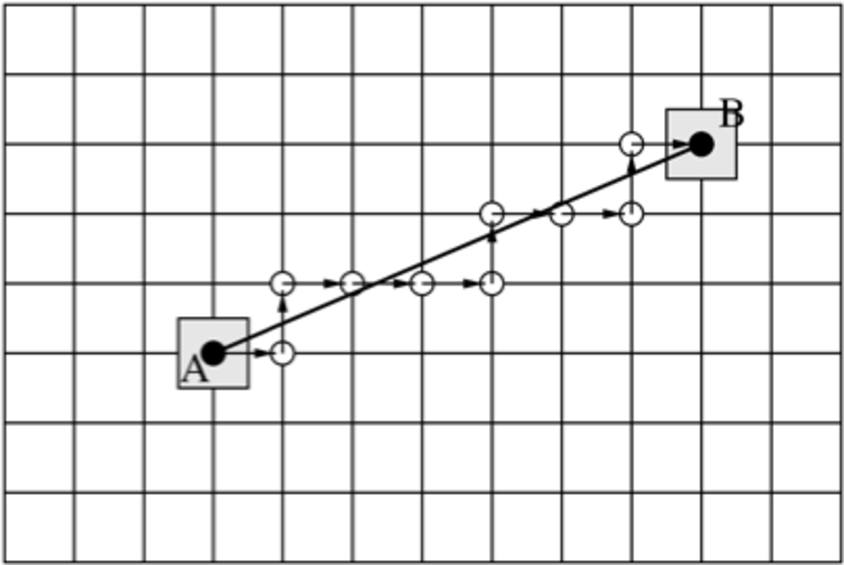
\includegraphics[width=0.5\textwidth]{media/linetrace.pdf}
  \caption{\label{line-trace} Tracing line through grid}
\end{figure}

An ultrasonic distance sensor mounted on a servomotor was used to check five different directions relative to the robot. Checking forward, and twice to each side with a set angle between each, this is similar to the vision based obstacle avoidance. This was planned to be used as a secondary method of avoiding obstacles, but turned out to be more effective, so when the values are combined it accounts for the stronger belief in the ultrasonic readings.

\begin{figure}[tbp]
  \centering
  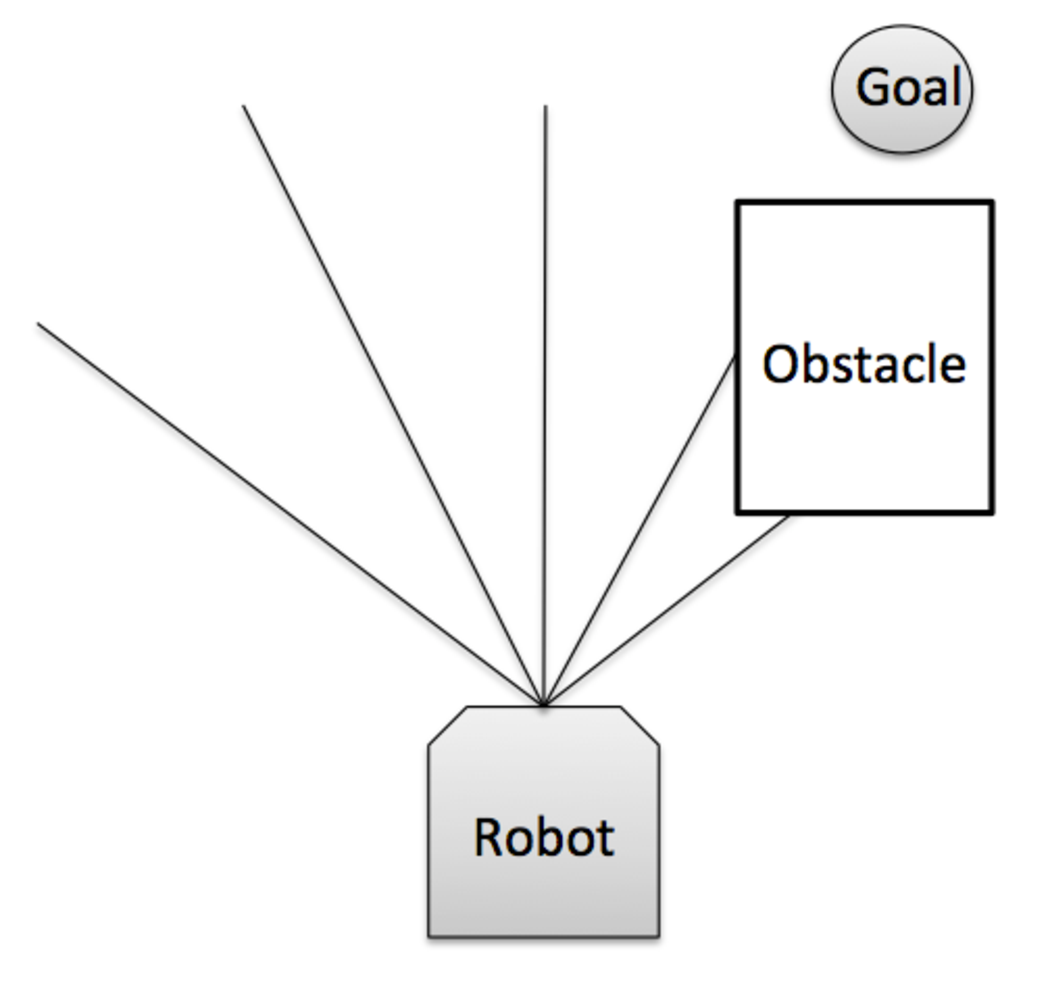
\includegraphics[width=0.5\textwidth]{media/rays.pdf}
  \caption{\label{policy-rays} Rays checked}
\end{figure}
\section{Machine Learning}
\label{section::learning}

This approach is based on on-policy policy iteration, but a greedy twist was added for computational simplicity. We do not iterate over every possible policy in all possible states. The algorithm considers the current state of the robot. The robot will attempt to execute a move to improve its state, where the reward is the straight line distance to the goal without avoiding future objects. Five policies were set from the current position the robot could go. The actual motor movements are all smoothed by a PID controller. The algorithm does not iterate over all states saving the optimal policies for each state because the obstacles are not static, and the policies would need to be recalculated each time an obstacle moved. A decision was made to avoid any training time in order for the robot to work out of the box, and improve with time. The robot does not have any movement commands hardcoded, and it will work if the motor cables are swapped. The robot attempts a motor command and receives feedback when the vision sensor values are updated; if the move was not beneficial, the error in either distance or angle would have increased. When the robot tries to turn left but the change in angle moves in the wrong direction, the PID controller will compensate for this and the robot will turn in the correct direction.

\section{Future Improvements}
\label{section::future}

Several future improvements could be made, three possible future enhancements are presented. First, add a more robust path planning algorithm. We went for keeping it simple. In our environment, we knew our greedy approach would work fast enough because of the simple box obstacles that needed to be avoided. In a more complex maze environment it is possible for our algorithm to fail and our robot to get stuck. Second, separate the code to a completely parallel implementation. It would be more efficient to have the vision processes, path planning and object avoidance all running as separate processes. This could be implemented by using the libraries provided by the Robot Operating System (ROS \footnote{\url{http://www.ros.org}} ) to pass data between different processes in a simple manner. The communication infrastructure provided by ROS would allow for the vision to be running continuously publishing the robot’s location, while the path planning, object avoiding and line tracing all run concurrently instead of in sequence. Finally, it would be beneficial to add more machine learning methods\cite{i2ml}\cite{ttml}, or a flexible controller architecture\cite{i2amr}. This would enable the swapping of controllers in order to compare different machine learning methods. For our project, we chose the one that would work with our time constraints. 

\section{Conclusion}
\label{section::conclusion}

We presented our project and our approach to the class and were pleased with our results. In the two runs we reached the goal on the first trial, and not on the second trial. In our final dozen tests, we managed to reach the goal in three quarters of the tests. We saw that the robot worked when commencing from any starting position and we were satisfied with these results in trials leading up to the final presentation. We were content with the simplicity of our solution. It proved to be more robust than other methods that relied on large training sets or hard coded camera transforms correcting skewing around the image edges. Our simple solution was designed to be robust and easy to use anywhere on any machine in as little time as possible. 



%%% REFERENCES %%%
\bibliographystyle{plain}
\bibliography{finalpaperrefs}
%\bibliographystyle{splncs}



%%% APPENDIX %%%

\end{document}





